\documentclass{beamer}
\usetheme[alternativetitlepage=true]{Torino}
\usepackage{listings}
\usepackage{hyperref}
\graphicspath{ {images/}}

\author{Scott Moser}
\title{Shell Script\^H\^H\^H\^H\^HProgramming Tips}
\institute{Michigan!/usr/group}
\date{June 9, 2014}

\begin{document}

\begin{frame}[t,plain]
    \titlepage
\end{frame}

\begin{frame}
   \frametitle{The Plan}
   \begin{itemize}
      \item Why Shell Programming?
      \item From Script to Program?
      \item Shell Script Tips
      \item questions
   \end{itemize}
\end{frame}

\begin{frame}
   \frametitle{Replace You}
   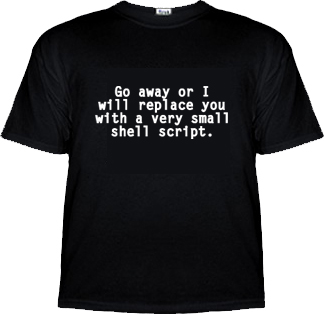
\includegraphics{replace-you}
\end{frame}

\begin{frame}
   \frametitle{Shell Programming?  What year is this!?}
   \begin{itemize}
      \item for I in perl python ruby python3; echo \$I replaced need for shell; done
      \item shell is cryptic, \$I is beautiful.
   \end{itemize}
\end{frame}

\begin{frame}
   \frametitle{Yes, Shell!}
   \begin{itemize}
      \item shell is *crazy fast* [scripts/bench-startup]
      \item even \href{https://gist.github.com/smoser/9780744}{/bin/bash is fast}.
      \item Ok, they're fast, but why do I care?
      \begin{itemize}
         \item your system load is 200, figure out why.
         \item tab completion
         \item boot time (hint, boot uses a lot of shell). 180 forks to init. 1059 to rc.local
      \end{itemize}
   \end{itemize}
\end{frame}

\begin{frame}
   \frametitle{Why Else?}
   \begin{itemize}
      \item copy and pasteable
   \end{itemize}
\end{frame}

\begin{frame}
   \frametitle Shell Scripting to Shell Programming
   \begin{itemize}
      \item functions and return values
      \item set -f
      \item newscript
      \item getopt
   \end{itemize}
\end{frame}

\begin{frame}
   \frametitle Tips and tricks
   \begin{itemize}
      \item ARRAYS!
      \item hashes
   \end{itemize}
\end{frame}

\begin{frame}
   \frametitle Why bash?
   \begin{itemize}
      \item real arrays
      \item \${HOME//e/ie}
      \item for((i=0;i<10;i++)); do echo \$i; done
      \item ARRAYS!
      \item hashes
      \item better trap
      \item \$RANDOM
      \item \$SECONDS
   \end{itemize}
\end{frame}


\end{document}
